\section{Muros}

Muros são estruturas realizadas com a finalidade de conter a movimentação do solo em cortes ou aterro de terrenos. São projetados quando a inclinação do talude em relação a horizontal é superior a 70º, e são compostos por reforço, aterro e elementos da face.

Os muros podem ser reforçados externamente ou internamente. Muros reforçados externamente são por exemplo muro de arrimo e muros de gravidade, em que o solo é apenas uma sobrecarga. Muros reforçados internamente, por outro lado, consideram o solo não apenas como material de construção para o muro como também se beneficiam da resistência do solo para compor a estrutura, como é o caso de muros de aterro reforçado com geossintéticos.

A ideia de introduzir uniformemente elementos de reforço no interior do material de aterro de um muro de suporte,  fez com que a concepção tradicional de estruturas de suporte de terras fosse alterada, sendo cada vez mais estudadas soluções atrativas visualmente e que não têm os aspetos de segurança e econômico como únicas preocupações. O primeiro muro de solo reforçado da era moderna foi proposto por Henri Vidal, em 1966, em que apresentou o conceito moderno de reforço de solo \cite{vidal:article}, composto por unidades verticais de face flexíveis e longas tiras metálicas colocadas na posição horizontal, e espaçadas horizontal e verticalmente, num aterro granular. 

As primeiras experiências de geossintéticos em taludes e muros de solo reforçado foram estabelecidas em 1981, com geogrelhas, nos Estados Unidos. “Atualmente, a utilização de inclusões de geossintéticos em taludes e muros de solo reforçado tem crescido acentuadamente, principalmente por representar uma alternativa, em geral, econômica e de fácil execução \cite{elias:article}.”

A Figura \ref{fig:face-muro} é referente a uma obra no interior de São Paulo, um muro que chega a até 12 metros de altura, com comprimento total do reforço de 20 metros.

\begin{figure}[htb]
 \caption{Face de um muro de solo reforçado com geogrelha}
 \label{fig:face-muro}
 \centering
 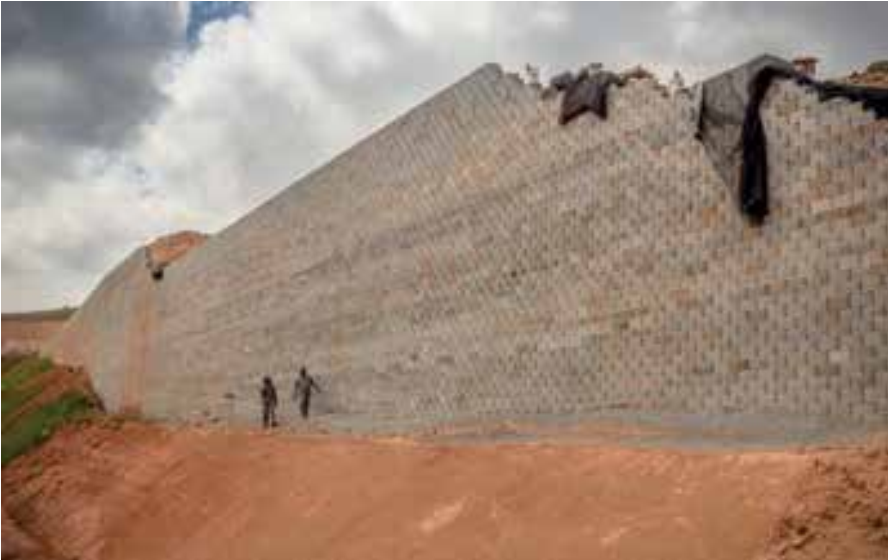
\includegraphics[scale=0.55]{face-muro.PNG}
 \fdireta{lavoie:artigo}
\end{figure}

Um estudo feito em 2001 pelo Departamento de Transporte dos Estados Unidos comparou os custos de execução de algumas soluções de contenção, levando em consideração a altura do muro a ser construído (Figura \ref{fig:custos-muros}. Segundo o estudo, fica clara as vantagens das estruturas de contenção em solos reforçados. Elas são soluções econômicas, capazes de apresentar grande tolerância a recalques de fundações, facilidade construtiva e prazo de execução reduzido. Pode-se acrescentar ainda a vantagem de não exigirem mão de obra especializada.

\begin{figure}[htb]
 \caption{Custos de construção, por área de face, em função da altura do muro, para várias soluções de contenção}
 \label{fig:custos-muros}
 \centering
 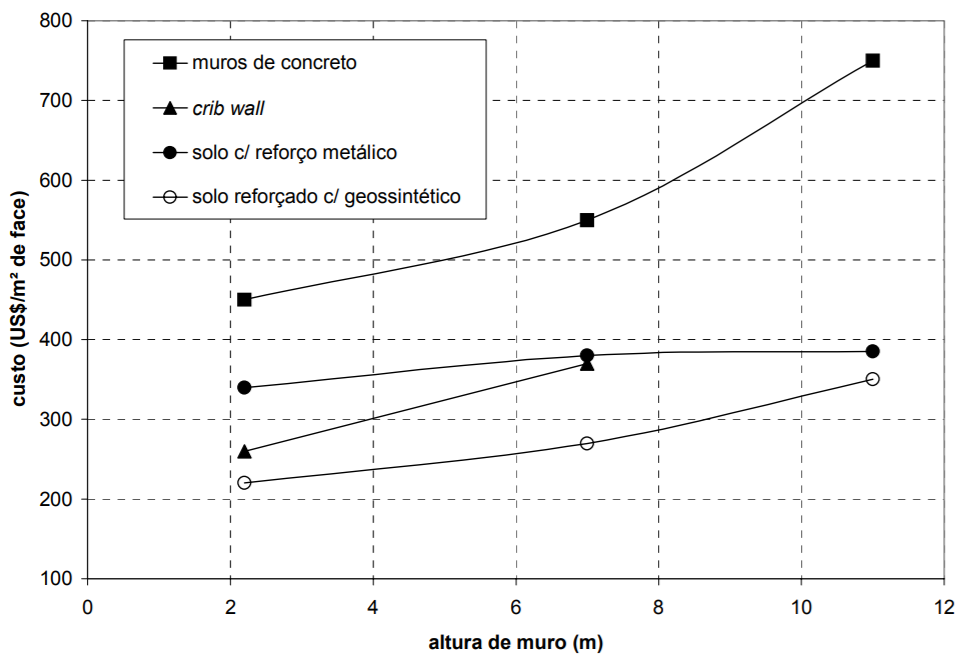
\includegraphics[scale=0.65]{custos-muros.PNG}
 \fdireta{elias:article}
\end{figure}

\section{Resíduos de Construção e Demolição (RCD)}

O ramo da construção civil é um dos mais vastos que compõem a indústria de um país. No Brasil, a construção civil é responsável por gerar mais de 220 mil toneladas de resíduos sólidos urbanos por dia, de acordo com o Panorama de Resíduos Sólidos publicado pela Associação Brasileira de Empresas de Limpeza Pública e Resíduos Especiais(ABRELPE), de 2016. 

Os resíduos sólidos da construção civil são regulamentados pela Política Nacional de Resíduos Sólidos (PNRS) e a Resolução 307/2002 do \sigla{CONAMA}{Conselho Nacional do Meio Ambiente}. A Resolução CONAMA 307 atribui responsabilidade compartilhada sob os resíduos sólidos da construção civil aos geradores, transportadores e gestores municipais.

A definição de RCD, de acordo com o CONAMA, é a seguinte: 

\begin{citacao}
Resíduos de construção civil: são os provenientes de construções, reformas, reparos e demolições de obras de construção civil, e os resultantes da preparação e da escavação de terrenos, tais como: tijolos, blocos cerâmicos, concreto em geral, solos, rochas, metais, resinas, colas, tintas, madeiras e compensados, forros, argamassa, gesso, telhas, pavimento asfáltico, vidros, plásticos, tubulações, fiação elétrica etc., comumente chamados de entulhos de obras, caliça ou metralha \cite{conama:algpseudocode}.
\end{citacao}

A composição dos resíduos sólidos da construção civil é classificada conforme a tabela  \ref{tabela:composicao_residuos_solidos} a seguir, de acordo com as possibilidades de reciclagem.

\begin{table}[htb]
\IBGEtab{%
  \caption{Composição dos resíduos sólidos da construção civil} \label{tabela:composicao_residuos_solidos}
}{%
\begin{tabular}{c|p{6cm}|p{6cm}}        
\toprule
Classe  & Descrição do resíduo & Exemplo   \\ \midrule \midrule
A       
& Materiais que podem ser reciclados ou reutilizados como agregado em obras de infraestrutura, edificações e canteiro de obras.          
& Tijolos, telhas e revestimentos cerâmicos; blocos e tubos de concreto e argamassa. \\ \midrule 
B       
& Materiais que podem ser reciclados e ganhar outras destinações.       
&  Vidro, gesso, madeira, plástico, papelão e outros. \\ \midrule 
C       
& Itens para o qual não existe ou não é viável aplicação econômica para recuperação ou reciclagem.        
&  Estopas, lixas, panos e pincéis desde que não tenham contato com substância que o classifique como D. \\ \midrule 
D       
& Aqueles compostos ou em contato de materiais/substâncias nocivos à saúde.        
&   Solvente e tintas; telhas e materiais de amianto; entulho de reformas em clínicas e instalações industriais que possam estar contaminados. \\ \bottomrule
\end{tabular}
}{%
  \fdireta{conama:algpseudocode}%
  }
\end{table}

A falta de políticas eficientes para a reciclagem e utilização dos resíduos de construção fazem com que a maior parte seja disposto inadequadamente. O RCD disposto inadequadamente polui o solo, deteriora a paisagem urbana, e constitui uma séria ameaça a saúde pública, além de oferecer abrigo para muitas espécies de vetores patogênicos, tais como: ratos, baratas, moscas, vermes, bactérias, fungos e vírus \cite{schneider:master}.

Na cidade de São Carlos, a quantidade de resíduos gerados varia de 250 a 450 ton/dia. Na maioria das vezes, o resíduo de construção civil é disposto em aterros de inertes, reduzindo a vida útil do aterro e degradando o meio ambiente, e em outras situações o resíduo é retirado das obras e disposto clandestinamente em locais como terrenos baldios, margens de rios e de ruas das periferias da Cidade de São Carlos. A Prefeitura compromete recursos, nem sempre mensuráveis, para a remoção ou tratamento desse resíduo.

A PROHAB São Carlos, em atendimento ao Plano Integrado de Gerenciamento de Resíduos de Construção Civil, e através do Programa de Sustentabilidade Ambiental e Social, implantou a Usina de Reciclagem de Resíduos da Construção Civil, inaugurada em dezembro de 2006. O projeto ainda conta com uma fascinante integração social, pois conta com a mão-de-obra de reeducandos da penitenciária Dr. Antônio de Queiroz Filho, do município de Itirapina.

A capacidade de produção da usina é de até 160 ton/dia, a usina não é capaz então de reciclar todo o resíduo gerado pelo município de São Carlos, mas ameniza o problema da disposição irregular. Além do benefício social e ambiental da usina, números mostram  que a produção de agregados com base no resíduo pode gerar economias de mais de 80\% em relação aos preços dos agregados convencionais, e que a partir deste material é possível fabricar componentes com uma economia de até 70\% em relação a similares com matéria-prima não reciclada \cite{prohab:site}.


\section{Reforços de Geossintéticos}

Geossintéticos são produtos industrializados com um ou mais componentes fabricado com polímero sintético ou natural. São especialmente fabricados para serem utilizados em aplicações geotécnicas, hidráulicas, ambientais e de transporte. Geossintéticos (Figura \ref{fig:amostras-geossinteticos}) podem ser responsáveis por diversas funções em uma estrutura, como separação, filtração, drenagem, e, como utilizado no a construção de muros, função de reforço. 

Em estruturas de solo reforçado (ESR) o reforço de geossintético atua de maneira semelhante às armaduras de aço em uma viga de concreto armado, ou seja, é responsável por restringir as deformações e aumentar a resistência do maciço, deve conferir em particular a resistência à tração.

Segundo \cite{manual-geossinteticos}, são inúmeras as vantagens de execução de geossintéticos como elemento de reforço:

\begin{itemize}
    \item Possibilita a construção de taludes e aterros com inclinação acentuadas;
    \item Minimiza o impacto ambiental decorrente das obras de contenção;
    \item Permite a adoção de tipos variados de acabamento da face dos taludes;
    \item Permite a execução de obras em locais de difícil acesso;
    \item Permite o uso de mão de obra não qualificada e equipamentos simples;
    \item Reduz consideravelmente o tempo de construção da obra.
\end{itemize}

\begin{figure}[htb]
 \caption{Amostras de geossintéticos}
 \label{fig:amostras-geossinteticos}
 \centering
 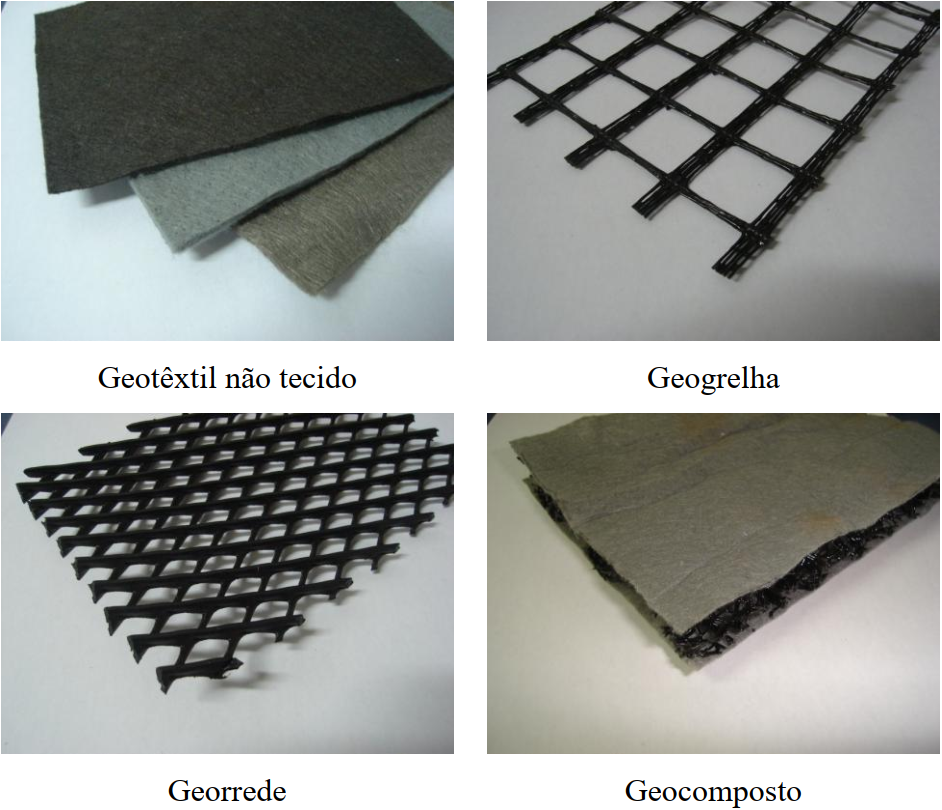
\includegraphics[scale=0.6]{amostras-geossinteticos.PNG}
 \fdireta{santos:2011:master}
\end{figure}


